% Options for packages loaded elsewhere
% Options for packages loaded elsewhere
\PassOptionsToPackage{unicode}{hyperref}
\PassOptionsToPackage{hyphens}{url}
%
\documentclass[
  ignorenonframetext,
  aspectratio=169,
  russian,
]{beamer}
\newif\ifbibliography
\usepackage{pgfpages}
\setbeamertemplate{caption}[numbered]
\setbeamertemplate{caption label separator}{: }
\setbeamercolor{caption name}{fg=normal text.fg}
\beamertemplatenavigationsymbolshorizontal
% Prevent slide breaks in the middle of a paragraph
\widowpenalties 1 10000
\raggedbottom
\AtBeginPart{
  \frame{\partpage}
}
\AtBeginSection{
  \ifbibliography
  \else
    \frame{\sectionpage}
  \fi
}
\AtBeginSubsection{
  \frame{\subsectionpage}
}
\usepackage{iftex}
\ifPDFTeX
  \usepackage[T1]{fontenc}
  \usepackage[utf8]{inputenc}
  \usepackage{textcomp} % provide euro and other symbols
\else % if luatex or xetex
  \usepackage{unicode-math} % this also loads fontspec
  \defaultfontfeatures{Scale=MatchLowercase}
  \defaultfontfeatures[\rmfamily]{Ligatures=TeX,Scale=1}
\fi
\usepackage{lmodern}

\usetheme[]{Montpellier}
\usecolortheme[]{seagull}
\ifPDFTeX\else
  % xetex/luatex font selection
\fi
% Use upquote if available, for straight quotes in verbatim environments
\IfFileExists{upquote.sty}{\usepackage{upquote}}{}
\IfFileExists{microtype.sty}{% use microtype if available
  \usepackage[]{microtype}
  \UseMicrotypeSet[protrusion]{basicmath} % disable protrusion for tt fonts
}{}

\usepackage{color}
\usepackage{fancyvrb}
\newcommand{\VerbBar}{|}
\newcommand{\VERB}{\Verb[commandchars=\\\{\}]}
\DefineVerbatimEnvironment{Highlighting}{Verbatim}{commandchars=\\\{\}}
% Add ',fontsize=\small' for more characters per line
\usepackage{framed}
\definecolor{shadecolor}{RGB}{241,243,245}
\newenvironment{Shaded}{\begin{snugshade}}{\end{snugshade}}
\newcommand{\AlertTok}[1]{\textcolor[rgb]{0.68,0.00,0.00}{#1}}
\newcommand{\AnnotationTok}[1]{\textcolor[rgb]{0.37,0.37,0.37}{#1}}
\newcommand{\AttributeTok}[1]{\textcolor[rgb]{0.40,0.45,0.13}{#1}}
\newcommand{\BaseNTok}[1]{\textcolor[rgb]{0.68,0.00,0.00}{#1}}
\newcommand{\BuiltInTok}[1]{\textcolor[rgb]{0.00,0.23,0.31}{#1}}
\newcommand{\CharTok}[1]{\textcolor[rgb]{0.13,0.47,0.30}{#1}}
\newcommand{\CommentTok}[1]{\textcolor[rgb]{0.37,0.37,0.37}{#1}}
\newcommand{\CommentVarTok}[1]{\textcolor[rgb]{0.37,0.37,0.37}{\textit{#1}}}
\newcommand{\ConstantTok}[1]{\textcolor[rgb]{0.56,0.35,0.01}{#1}}
\newcommand{\ControlFlowTok}[1]{\textcolor[rgb]{0.00,0.23,0.31}{\textbf{#1}}}
\newcommand{\DataTypeTok}[1]{\textcolor[rgb]{0.68,0.00,0.00}{#1}}
\newcommand{\DecValTok}[1]{\textcolor[rgb]{0.68,0.00,0.00}{#1}}
\newcommand{\DocumentationTok}[1]{\textcolor[rgb]{0.37,0.37,0.37}{\textit{#1}}}
\newcommand{\ErrorTok}[1]{\textcolor[rgb]{0.68,0.00,0.00}{#1}}
\newcommand{\ExtensionTok}[1]{\textcolor[rgb]{0.00,0.23,0.31}{#1}}
\newcommand{\FloatTok}[1]{\textcolor[rgb]{0.68,0.00,0.00}{#1}}
\newcommand{\FunctionTok}[1]{\textcolor[rgb]{0.28,0.35,0.67}{#1}}
\newcommand{\ImportTok}[1]{\textcolor[rgb]{0.00,0.46,0.62}{#1}}
\newcommand{\InformationTok}[1]{\textcolor[rgb]{0.37,0.37,0.37}{#1}}
\newcommand{\KeywordTok}[1]{\textcolor[rgb]{0.00,0.23,0.31}{\textbf{#1}}}
\newcommand{\NormalTok}[1]{\textcolor[rgb]{0.00,0.23,0.31}{#1}}
\newcommand{\OperatorTok}[1]{\textcolor[rgb]{0.37,0.37,0.37}{#1}}
\newcommand{\OtherTok}[1]{\textcolor[rgb]{0.00,0.23,0.31}{#1}}
\newcommand{\PreprocessorTok}[1]{\textcolor[rgb]{0.68,0.00,0.00}{#1}}
\newcommand{\RegionMarkerTok}[1]{\textcolor[rgb]{0.00,0.23,0.31}{#1}}
\newcommand{\SpecialCharTok}[1]{\textcolor[rgb]{0.37,0.37,0.37}{#1}}
\newcommand{\SpecialStringTok}[1]{\textcolor[rgb]{0.13,0.47,0.30}{#1}}
\newcommand{\StringTok}[1]{\textcolor[rgb]{0.13,0.47,0.30}{#1}}
\newcommand{\VariableTok}[1]{\textcolor[rgb]{0.07,0.07,0.07}{#1}}
\newcommand{\VerbatimStringTok}[1]{\textcolor[rgb]{0.13,0.47,0.30}{#1}}
\newcommand{\WarningTok}[1]{\textcolor[rgb]{0.37,0.37,0.37}{\textit{#1}}}

\usepackage{longtable,booktabs,array}
\usepackage{calc} % for calculating minipage widths
\usepackage{caption}
% Make caption package work with longtable
\makeatletter
\def\fnum@table{\tablename~\thetable}
\makeatother
\usepackage{graphicx}
\makeatletter
\newsavebox\pandoc@box
\newcommand*\pandocbounded[1]{% scales image to fit in text height/width
  \sbox\pandoc@box{#1}%
  \Gscale@div\@tempa{\textheight}{\dimexpr\ht\pandoc@box+\dp\pandoc@box\relax}%
  \Gscale@div\@tempb{\linewidth}{\wd\pandoc@box}%
  \ifdim\@tempb\p@<\@tempa\p@\let\@tempa\@tempb\fi% select the smaller of both
  \ifdim\@tempa\p@<\p@\scalebox{\@tempa}{\usebox\pandoc@box}%
  \else\usebox{\pandoc@box}%
  \fi%
}
% Set default figure placement to htbp
\def\fps@figure{htbp}
\makeatother



\ifLuaTeX
\usepackage[bidi=basic,provide=*]{babel}
\else
\usepackage[bidi=default,provide=*]{babel}
\fi
% get rid of language-specific shorthands (see #6817):
\let\LanguageShortHands\languageshorthands
\def\languageshorthands#1{}


\setlength{\emergencystretch}{3em} % prevent overfull lines

\providecommand{\tightlist}{%
  \setlength{\itemsep}{0pt}\setlength{\parskip}{0pt}}



 

\usepackage[]{csquotes}

\usepackage{libertine}
\makeatletter
\@ifpackageloaded{caption}{}{\usepackage{caption}}
\AtBeginDocument{%
\ifdefined\contentsname
  \renewcommand*\contentsname{Содержание}
\else
  \newcommand\contentsname{Содержание}
\fi
\ifdefined\listfigurename
  \renewcommand*\listfigurename{Список иллюстраций}
\else
  \newcommand\listfigurename{Список иллюстраций}
\fi
\ifdefined\listtablename
  \renewcommand*\listtablename{Список таблиц}
\else
  \newcommand\listtablename{Список таблиц}
\fi
\ifdefined\figurename
  \renewcommand*\figurename{Рисунок}
\else
  \newcommand\figurename{Рисунок}
\fi
\ifdefined\tablename
  \renewcommand*\tablename{Таблица}
\else
  \newcommand\tablename{Таблица}
\fi
}
\@ifpackageloaded{float}{}{\usepackage{float}}
\floatstyle{ruled}
\@ifundefined{c@chapter}{\newfloat{codelisting}{h}{lop}}{\newfloat{codelisting}{h}{lop}[chapter]}
\floatname{codelisting}{Список}
\newcommand*\listoflistings{\listof{codelisting}{Листинги}}
\makeatother
\makeatletter
\makeatother
\makeatletter
\@ifpackageloaded{caption}{}{\usepackage{caption}}
\@ifpackageloaded{subcaption}{}{\usepackage{subcaption}}
\makeatother

\usepackage{bookmark}
\IfFileExists{xurl.sty}{\usepackage{xurl}}{} % add URL line breaks if available
\urlstyle{same}
\hypersetup{
  pdftitle={Лабораторная работа №4},
  pdfauthor={Mohamed Musa},
  pdflang={ru-RU},
  hidelinks,
  pdfcreator={LaTeX via pandoc}}


\title{Лабораторная работа №4}
\subtitle{Продвинутое использование git}
\author{Mohamed Musa}
\date{2025-10-09}

\begin{document}
\frame{\titlepage}

\renewcommand*\contentsname{Содержание}
\begin{frame}[allowframebreaks]
  \frametitle{Содержание}
  \setcounter{tocdepth}{2}
  \tableofcontents
\end{frame}
\setcounter{tocdepth}{2}
\tableofcontents
}

\section{1. Информация}\label{ux438ux43dux444ux43eux440ux43cux430ux446ux438ux44f}

\begin{frame}{1.1 Докладчик}
\phantomsection\label{ux434ux43eux43aux43bux430ux434ux447ux438ux43a}
\begin{columns}[c]
\begin{column}{0.7\linewidth}
\begin{itemize}[<+->]
\tightlist
\item
  Mohamed Musa
\item
  Студент группы НКАбд-05-24
\item
  Студенческий билет: 1032248286
\item
  Российский университет дружбы народов
\item
  \href{mailto:1032248286@pfur.ru}{\nolinkurl{1032248286@pfur.ru}}
\end{itemize}
\end{column}

\begin{column}{0.3\linewidth}
\pandocbounded{
\includegraphics[keepaspectratio]{./image/kulyabov.jpg}}
\end{column}
\end{columns}
\end{frame}

\section{2. Вводная
часть}\label{ux432ux432ux43eux434ux43dux430ux44f-ux447ux430ux441ux442ux44c}

\begin{frame}{2.1 Актуальность}
\phantomsection\label{ux430ux43aux442ux443ux430ux43bux44cux43dux43eux441ux442ux44c}
\begin{itemize}[<+->]
\tightlist
\item
  Правильная организация работы с системой контроля версий критически
  важна для командной разработки
\item
  Git-flow предоставляет структурированный подход к ветвлению
\item
  Семантическое версионирование обеспечивает понятную систему нумерации
  релизов
\item
  Conventional commits стандартизируют историю изменений
\end{itemize}
\end{frame}

\begin{frame}{2.2 Объект и предмет исследования}
\phantomsection\label{ux43eux431ux44aux435ux43aux442-ux438-ux43fux440ux435ux434ux43cux435ux442-ux438ux441ux441ux43bux435ux434ux43eux432ux430ux43dux438ux44f}
\begin{itemize}[<+->]
\tightlist
\item
  Система контроля версий Git
\item
  Модель ветвления Gitflow
\item
  Инструменты автоматизации работы с репозиториями
\item
  Стандарты оформления коммитов и версионирования
\end{itemize}
\end{frame}

\begin{frame}{2.3 Цели и задачи}
\phantomsection\label{ux446ux435ux43bux438-ux438-ux437ux430ux434ux430ux447ux438}
\begin{itemize}[<+->]
\tightlist
\item
  Получить навыки работы с git-flow
\item
  Освоить семантическое версионирование
\item
  Научиться использовать conventional commits
\item
  Автоматизировать создание changelog
\end{itemize}
\end{frame}

\begin{frame}{2.4 Материалы и методы}
\phantomsection\label{ux43cux430ux442ux435ux440ux438ux430ux43bux44b-ux438-ux43cux435ux442ux43eux434ux44b}
\begin{itemize}[<+->]
\tightlist
\item
  Git и расширение git-flow
\item
  Node.js и пакетный менеджер pnpm
\item
  Инструменты: commitizen, standard-changelog
\item
  Тестовый репозиторий git-extended
\end{itemize}
\end{frame}

\section{3. Теоретические
сведения}\label{ux442ux435ux43eux440ux435ux442ux438ux447ux435ux441ux43aux438ux435-ux441ux432ux435ux434ux435ux43dux438ux44f}

\begin{frame}{3.1 Gitflow Workflow}
\phantomsection\label{gitflow-workflow}
\begin{itemize}[<+->]
\tightlist
\item
  Модель ветвления, опубликованная Винсентом Дриссеном
\item
  Строгая модель с учётом выпуска проекта
\item
  Основные ветки: \textbf{master} и \textbf{develop}
\item
  Вспомогательные ветки: \textbf{feature}, \textbf{release},
  \textbf{hotfix}
\end{itemize}
\end{frame}

\begin{frame}{3.2 Схема работы Gitflow}
\phantomsection\label{ux441ux445ux435ux43cux430-ux440ux430ux431ux43eux442ux44b-gitflow}
\begin{itemize}[<+->]
\tightlist
\item
  Из master создаётся develop
\item
  Из develop создаются feature ветки
\item
  Feature ветки сливаются обратно в develop
\item
  Из develop создаются release ветки
\item
  Release сливается в master и develop
\item
  Hotfix создаётся из master и сливается в обе ветки
\end{itemize}
\end{frame}

\begin{frame}[fragile]{3.3 Семантическое версионирование}
\phantomsection\label{ux441ux435ux43cux430ux43dux442ux438ux447ux435ux441ux43aux43eux435-ux432ux435ux440ux441ux438ux43eux43dux438ux440ux43eux432ux430ux43dux438ux435}
Формат версии: \textbf{МАЖОРНАЯ.МИНОРНАЯ.ПАТЧ}

\begin{itemize}[<+->]
\tightlist
\item
  \textbf{МАЖОРНАЯ} --- обратно несовместимые изменения API
\item
  \textbf{МИНОРНАЯ} --- новая функциональность с обратной совместимостью
\item
  \textbf{ПАТЧ} --- обратно совместимые исправления ошибок
\end{itemize}

Пример: \texttt{1.2.3} → \texttt{2.0.0} (breaking change)
\end{frame}

\begin{frame}[fragile]{3.4 Conventional Commits}
\phantomsection\label{conventional-commits}
Структура коммита:

\begin{verbatim}
<тип>(<область>): <описание>

[тело]

[нижний колонтитул]
\end{verbatim}
\end{frame}

\begin{frame}{3.5 Типы коммитов}
\phantomsection\label{ux442ux438ux43fux44b-ux43aux43eux43cux43cux438ux442ux43eux432}
\begin{itemize}[<+->]
\tightlist
\item
  \textbf{feat:} --- новая функция (MINOR)
\item
  \textbf{fix:} --- исправление ошибки (PATCH)
\item
  \textbf{docs:} --- изменения в документации
\item
  \textbf{style:} --- форматирование кода
\item
  \textbf{refactor:} --- рефакторинг
\item
  \textbf{test:} --- добавление тестов
\item
  \textbf{chore:} --- изменения в сборке
\end{itemize}
\end{frame}

\begin{frame}{3.6 Инструменты}
\phantomsection\label{ux438ux43dux441ux442ux440ux443ux43cux435ux43dux442ux44b}
\begin{itemize}[<+->]
\tightlist
\item
  \textbf{git-flow} --- расширение Git для Gitflow
\item
  \textbf{pnpm} --- быстрый пакетный менеджер
\item
  \textbf{commitizen} --- помощник для создания коммитов
\item
  \textbf{standard-changelog} --- генератор changelog \# Выполнение
  работы
\end{itemize}
\end{frame}

\begin{frame}{3.7 Установка программного обеспечения}
\phantomsection\label{ux443ux441ux442ux430ux43dux43eux432ux43aux430-ux43fux440ux43eux433ux440ux430ux43cux43cux43dux43eux433ux43e-ux43eux431ux435ux441ux43fux435ux447ux435ux43dux438ux44f}
Установлены следующие компоненты:

\begin{itemize}[<+->]
\tightlist
\item
  git-flow (из репозитория Copr)
\item
  Node.js и pnpm
\item
  commitizen (глобально через pnpm)
\item
  standard-changelog (глобально через pnpm)
\end{itemize}
\end{frame}

\begin{frame}[fragile]{3.8 Установка git-flow}
\phantomsection\label{ux443ux441ux442ux430ux43dux43eux432ux43aux430-git-flow}
Для Fedora:

\begin{Shaded}
\begin{Highlighting}[]
\ExtensionTok{dnf}\NormalTok{ copr enable elegos/gitflow}
\ExtensionTok{dnf}\NormalTok{ install gitflow}
\end{Highlighting}
\end{Shaded}
\end{frame}

\begin{frame}[fragile]{3.9 Установка Node.js}
\phantomsection\label{ux443ux441ux442ux430ux43dux43eux432ux43aux430-node.js}
Установка необходимых пакетов:

\begin{Shaded}
\begin{Highlighting}[]
\ExtensionTok{dnf}\NormalTok{ install nodejs}
\ExtensionTok{dnf}\NormalTok{ install pnpm}
\end{Highlighting}
\end{Shaded}
\end{frame}

\begin{frame}[fragile]{3.10 Настройка pnpm}
\phantomsection\label{ux43dux430ux441ux442ux440ux43eux439ux43aux430-pnpm}
Выполнена настройка pnpm package manager:

\begin{Shaded}
\begin{Highlighting}[]
\ExtensionTok{pnpm}\NormalTok{ setup}
\BuiltInTok{source}\NormalTok{ \textasciitilde{}/.bashrc}
\end{Highlighting}
\end{Shaded}
\end{frame}

\begin{frame}{3.11 Настройка pnpm (скриншот)}
\phantomsection\label{ux43dux430ux441ux442ux440ux43eux439ux43aux430-pnpm-ux441ux43aux440ux438ux43dux448ux43eux442}
\begin{figure}[H]

{\centering 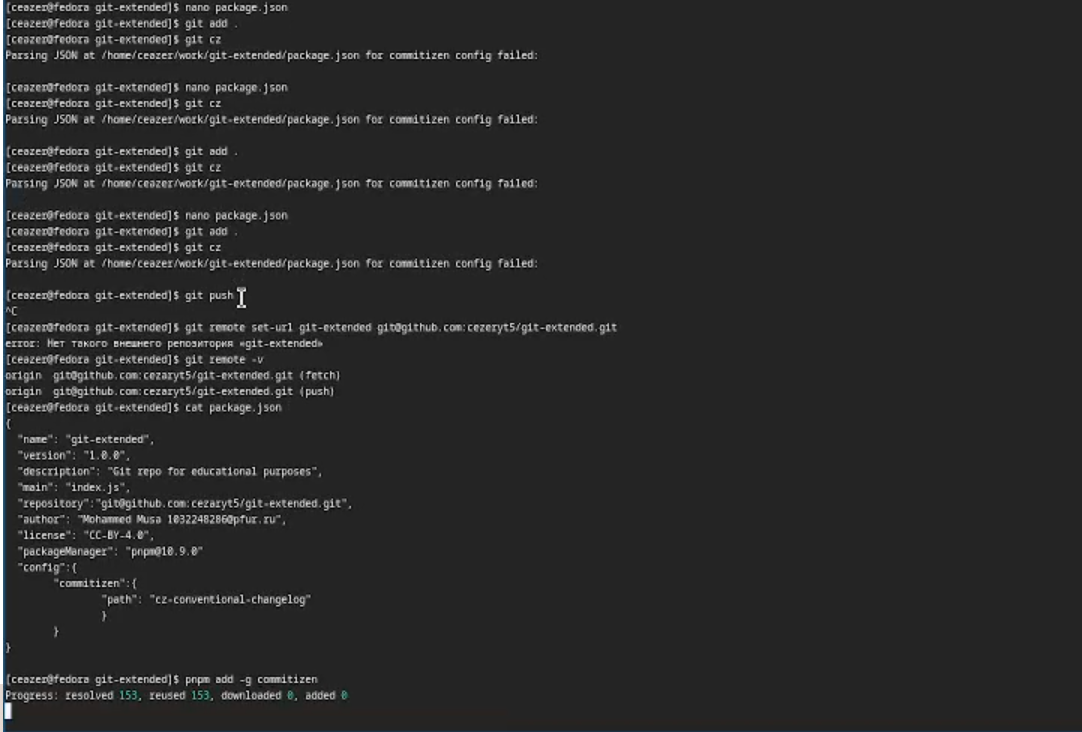
\includegraphics[width=0.8\linewidth,height=\textheight,keepaspectratio]{image/pnpm.png}

}

\caption{Настройка pnpm}

\end{figure}%
\end{frame}

\begin{frame}{3.12 Создание репозитория}
\phantomsection\label{ux441ux43eux437ux434ux430ux43dux438ux435-ux440ux435ux43fux43eux437ux438ux442ux43eux440ux438ux44f}
Выполнены следующие шаги:

\begin{enumerate}[<+->]
\tightlist
\item
  Создан репозиторий git-extended на GitHub
\item
  Инициализирован локальный репозиторий
\item
  Выполнен первый коммит
\item
  Настроено подключение к удаленному репозиторию
\end{enumerate}
\end{frame}

\begin{frame}[fragile]{3.13 Конфигурация Node.js}
\phantomsection\label{ux43aux43eux43dux444ux438ux433ux443ux440ux430ux446ux438ux44f-node.js}
Инициализация проекта:

\begin{Shaded}
\begin{Highlighting}[]
\ExtensionTok{pnpm}\NormalTok{ init}
\end{Highlighting}
\end{Shaded}

Параметры:

\begin{itemize}[<+->]
\tightlist
\item
  Название: git-extended
\item
  Версия: 1.0.0
\item
  Лицензия: CC-BY-4.0
\item
  Автор: Mohamed Musa
\end{itemize}
\end{frame}

\begin{frame}[fragile]{3.14 Файл package.json}
\phantomsection\label{ux444ux430ux439ux43b-package.json}
Добавлена конфигурация для commitizen:

\begin{Shaded}
\begin{Highlighting}[]
\ErrorTok{"config":} \FunctionTok{\{}
    \DataTypeTok{"commitizen"}\FunctionTok{:} \FunctionTok{\{}
        \DataTypeTok{"path"}\FunctionTok{:} \StringTok{"cz{-}conventional{-}changelog"}
    \FunctionTok{\}}
\FunctionTok{\}}
\end{Highlighting}
\end{Shaded}
\end{frame}

\begin{frame}{3.15 Файл package.json (скриншот)}
\phantomsection\label{ux444ux430ux439ux43b-package.json-ux441ux43aux440ux438ux43dux448ux43eux442}
\begin{figure}[H]

{\centering 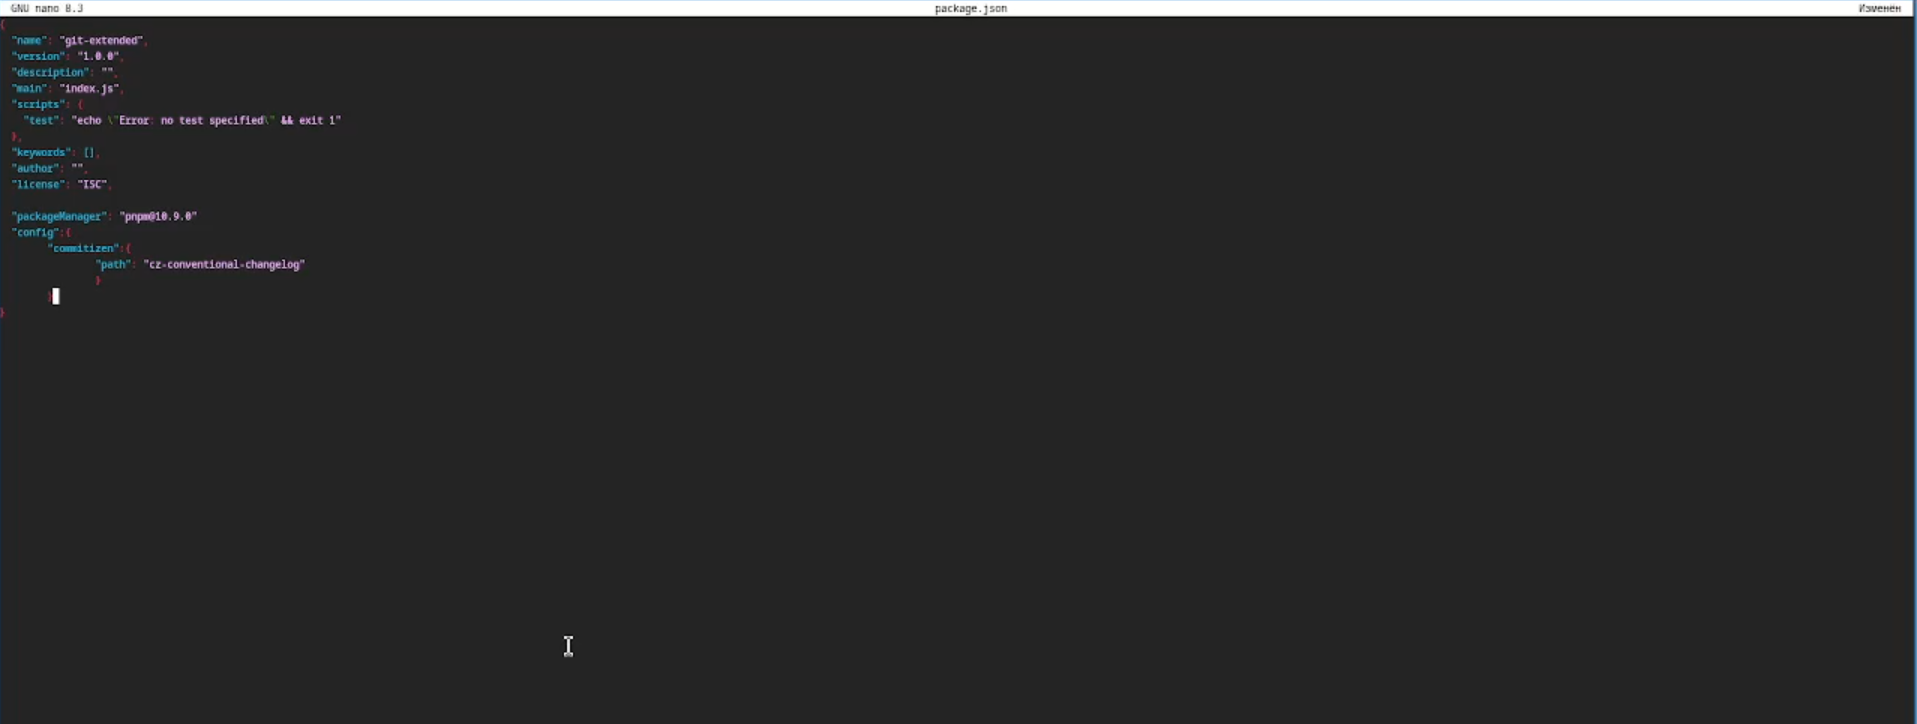
\includegraphics[width=0.8\linewidth,height=\textheight,keepaspectratio]{image/package.json.png}

}

\caption{Конфигурация package.json}

\end{figure}%
\end{frame}

\begin{frame}[fragile]{3.16 Установка commitizen}
\phantomsection\label{ux443ux441ux442ux430ux43dux43eux432ux43aux430-commitizen}
Установка инструментов для conventional commits:

\begin{Shaded}
\begin{Highlighting}[]
\ExtensionTok{pnpm}\NormalTok{ add }\AttributeTok{{-}g}\NormalTok{ commitizen}
\ExtensionTok{pnpm}\NormalTok{ add }\AttributeTok{{-}g}\NormalTok{ standard{-}changelog}
\end{Highlighting}
\end{Shaded}
\end{frame}

\begin{frame}{3.17 Установка commitizen (скриншот)}
\phantomsection\label{ux443ux441ux442ux430ux43dux43eux432ux43aux430-commitizen-ux441ux43aux440ux438ux43dux448ux43eux442}
\begin{figure}[H]

{\centering 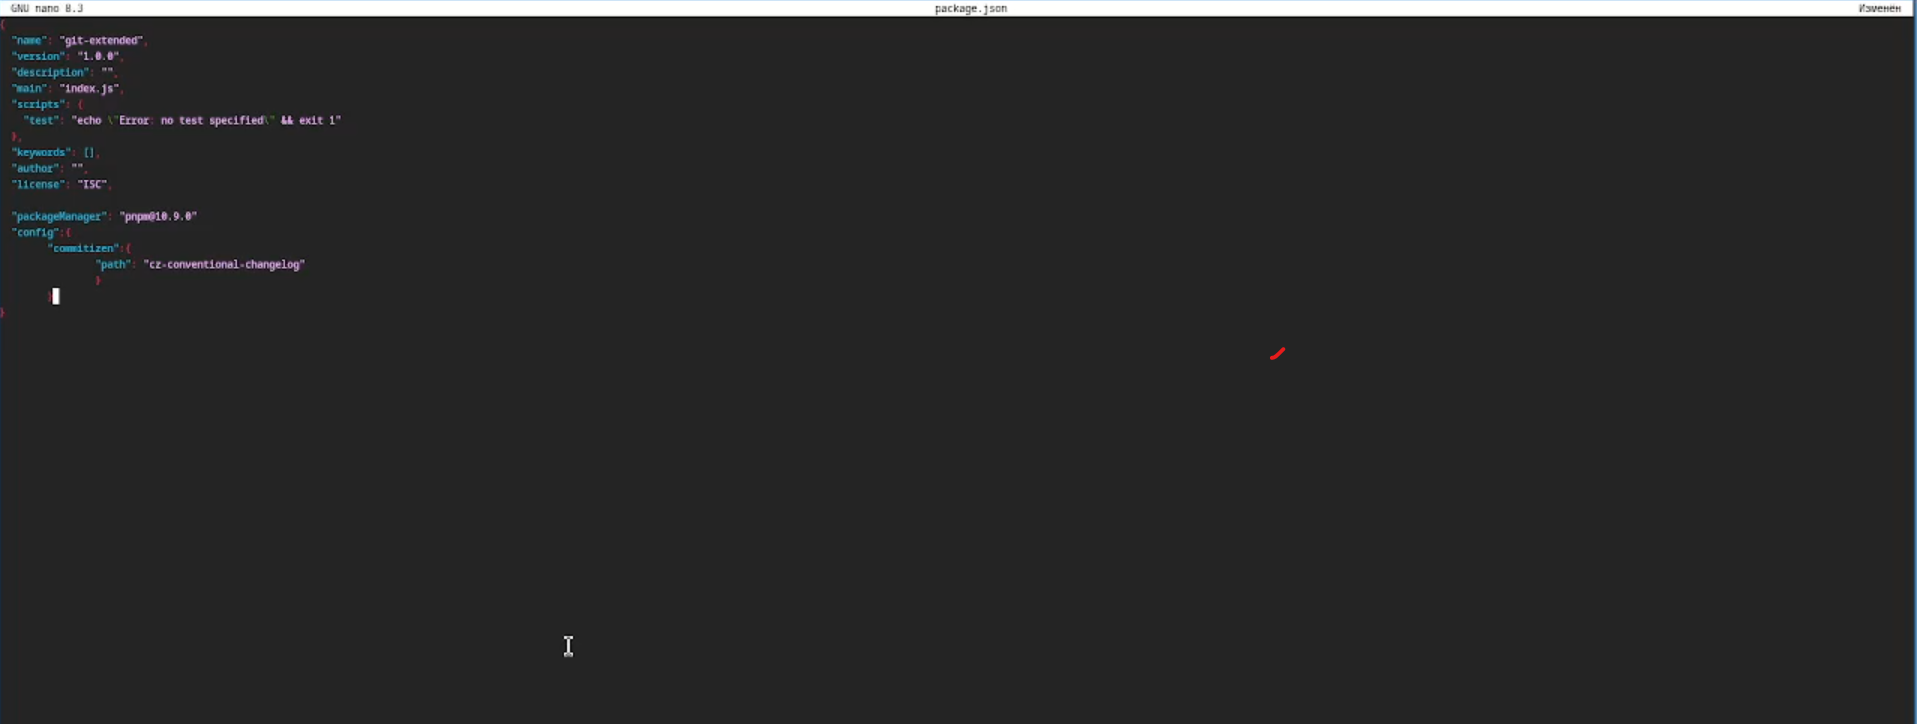
\includegraphics[width=0.8\linewidth,height=\textheight,keepaspectratio]{image/commitzen.png}

}

\caption{Установка commitizen}

\end{figure}%
\end{frame}

\begin{frame}[fragile]{3.18 Инициализация git-flow}
\phantomsection\label{ux438ux43dux438ux446ux438ux430ux43bux438ux437ux430ux446ux438ux44f-git-flow}
Команды инициализации:

\begin{Shaded}
\begin{Highlighting}[]
\FunctionTok{git}\NormalTok{ flow init}
\end{Highlighting}
\end{Shaded}

Параметры:

\begin{itemize}[<+->]
\tightlist
\item
  Префикс для тегов: \texttt{v}
\item
  Ветка production: master
\item
  Ветка разработки: develop
\end{itemize}
\end{frame}

\begin{frame}[fragile]{3.19 Загрузка веток на GitHub}
\phantomsection\label{ux437ux430ux433ux440ux443ux437ux43aux430-ux432ux435ux442ux43eux43a-ux43dux430-github}
\begin{Shaded}
\begin{Highlighting}[]
\FunctionTok{git}\NormalTok{ push }\AttributeTok{{-}{-}all}
\FunctionTok{git}\NormalTok{ branch }\AttributeTok{{-}{-}set{-}upstream{-}to}\OperatorTok{=}\NormalTok{origin/develop develop}
\end{Highlighting}
\end{Shaded}
\end{frame}

\begin{frame}[fragile]{3.20 Создание первого релиза}
\phantomsection\label{ux441ux43eux437ux434ux430ux43dux438ux435-ux43fux435ux440ux432ux43eux433ux43e-ux440ux435ux43bux438ux437ux430}
Команды для создания релиза 1.0.0:

\begin{Shaded}
\begin{Highlighting}[]
\FunctionTok{git}\NormalTok{ flow release start 1.0.0}
\ExtensionTok{standard{-}changelog} \AttributeTok{{-}{-}first{-}release}
\FunctionTok{git}\NormalTok{ add CHANGELOG.md}
\FunctionTok{git}\NormalTok{ commit }\AttributeTok{{-}am} \StringTok{\textquotesingle{}chore(site): add changelog\textquotesingle{}}
\FunctionTok{git}\NormalTok{ flow release finish 1.0.0}
\end{Highlighting}
\end{Shaded}
\end{frame}

\begin{frame}{3.21 Создание первого релиза (скриншот)}
\phantomsection\label{ux441ux43eux437ux434ux430ux43dux438ux435-ux43fux435ux440ux432ux43eux433ux43e-ux440ux435ux43bux438ux437ux430-ux441ux43aux440ux438ux43dux448ux43eux442}
\begin{figure}[H]

{\centering 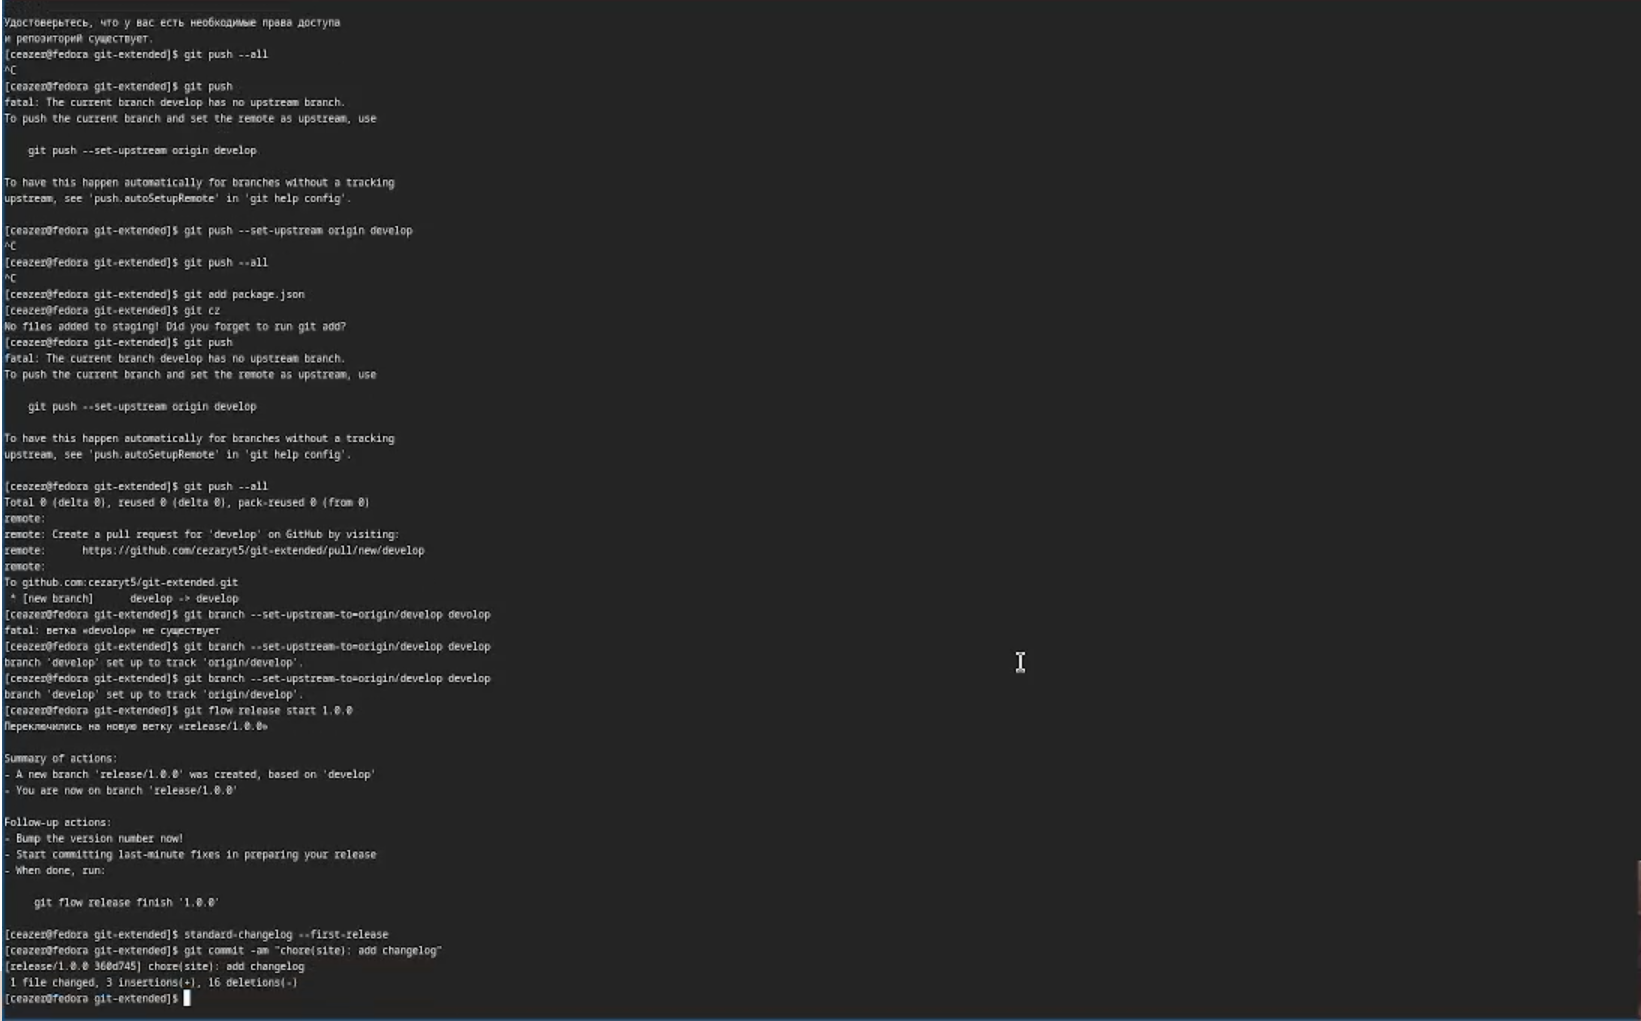
\includegraphics[width=0.8\linewidth,height=\textheight,keepaspectratio]{image/first release.png}

}

\caption{Процесс создания релиза 1.0.0}

\end{figure}%
\end{frame}

\begin{frame}[fragile]{3.22 Публикация релиза}
\phantomsection\label{ux43fux443ux431ux43bux438ux43aux430ux446ux438ux44f-ux440ux435ux43bux438ux437ux430}
Отправка на GitHub:

\begin{Shaded}
\begin{Highlighting}[]
\FunctionTok{git}\NormalTok{ push }\AttributeTok{{-}{-}all}
\FunctionTok{git}\NormalTok{ push }\AttributeTok{{-}{-}tags}
\ExtensionTok{gh}\NormalTok{ release create v1.0.0 }\AttributeTok{{-}F}\NormalTok{ CHANGELOG.md}
\end{Highlighting}
\end{Shaded}
\end{frame}

\begin{frame}[fragile]{3.23 Работа с changelog}
\phantomsection\label{ux440ux430ux431ux43eux442ux430-ux441-changelog}
Автоматическая генерация журнала изменений:

\begin{Shaded}
\begin{Highlighting}[]
\ExtensionTok{standard{-}changelog}
\end{Highlighting}
\end{Shaded}

Журнал содержит:

\begin{itemize}[<+->]
\tightlist
\item
  Список новых функций (feat)
\item
  Исправления ошибок (fix)
\item
  Другие изменения
\end{itemize}
\end{frame}

\begin{frame}{3.24 Работа с changelog (скриншот)}
\phantomsection\label{ux440ux430ux431ux43eux442ux430-ux441-changelog-ux441ux43aux440ux438ux43dux448ux43eux442}
\begin{figure}[H]

{\centering 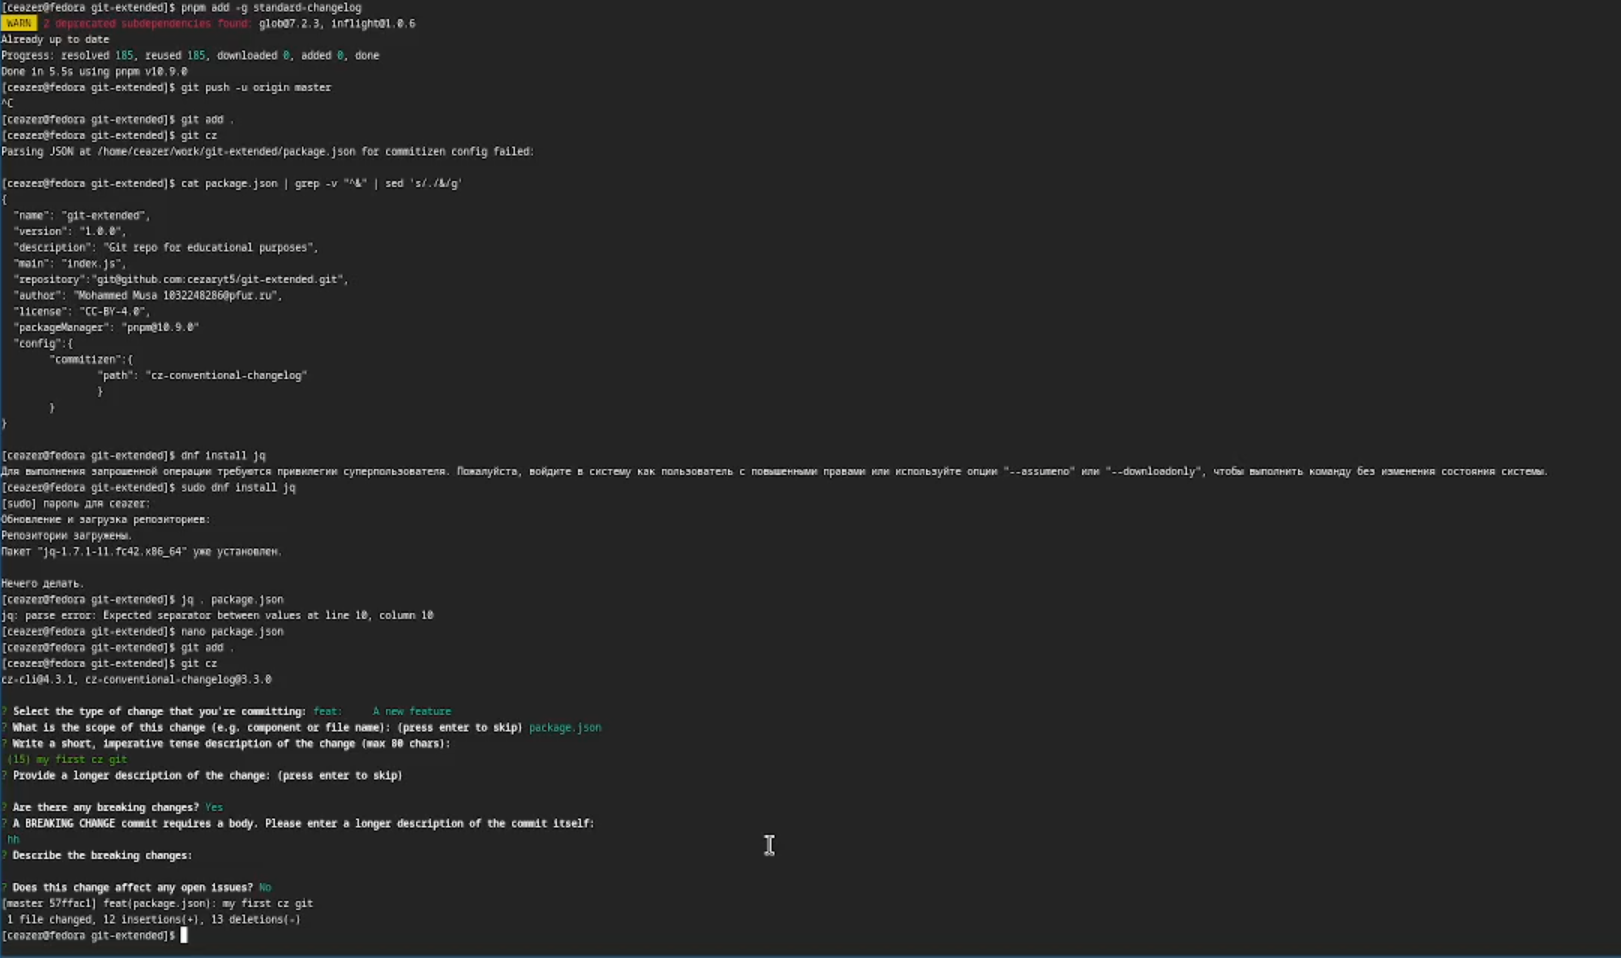
\includegraphics[width=0.8\linewidth,height=\textheight,keepaspectratio]{image/changelog.png}

}

\caption{Управление журналом изменений}

\end{figure}%
\end{frame}

\begin{frame}[fragile]{3.25 Добавление записей в changelog}
\phantomsection\label{ux434ux43eux431ux430ux432ux43bux435ux43dux438ux435-ux437ux430ux43fux438ux441ux435ux439-ux432-changelog}
Процесс обновления changelog при новом релизе:

\begin{Shaded}
\begin{Highlighting}[]
\FunctionTok{git}\NormalTok{ add CHANGELOG.md}
\FunctionTok{git}\NormalTok{ commit }\AttributeTok{{-}am} \StringTok{\textquotesingle{}chore(site): update changelog\textquotesingle{}}
\end{Highlighting}
\end{Shaded}
\end{frame}

\begin{frame}{3.26 Добавление записей в changelog (скриншот)}
\phantomsection\label{ux434ux43eux431ux430ux432ux43bux435ux43dux438ux435-ux437ux430ux43fux438ux441ux435ux439-ux432-changelog-ux441ux43aux440ux438ux43dux448ux43eux442}
\begin{figure}[H]

{\centering 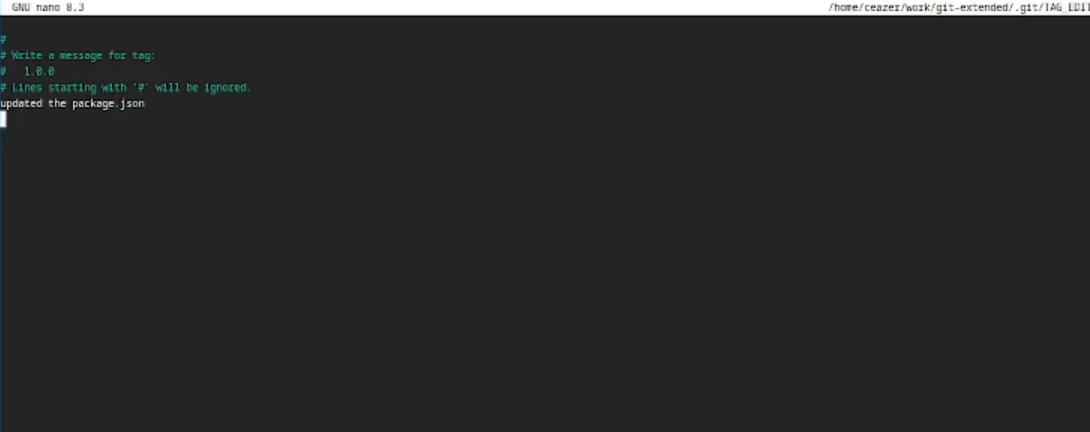
\includegraphics[width=0.8\linewidth,height=\textheight,keepaspectratio]{image/addChangelog.png}

}

\caption{Обновление changelog}

\end{figure}%
\end{frame}

\begin{frame}[fragile]{3.27 Разработка новой функциональности}
\phantomsection\label{ux440ux430ux437ux440ux430ux431ux43eux442ux43aux430-ux43dux43eux432ux43eux439-ux444ux443ux43dux43aux446ux438ux43eux43dux430ux43bux44cux43dux43eux441ux442ux438}
Работа с feature ветками:

\begin{Shaded}
\begin{Highlighting}[]
\FunctionTok{git}\NormalTok{ flow feature start feature\_branch}
\CommentTok{\# ... разработка ...}
\FunctionTok{git}\NormalTok{ flow feature finish feature\_branch}
\end{Highlighting}
\end{Shaded}
\end{frame}

\begin{frame}{3.28 Создание нового релиза}
\phantomsection\label{ux441ux43eux437ux434ux430ux43dux438ux435-ux43dux43eux432ux43eux433ux43e-ux440ux435ux43bux438ux437ux430}
Процесс создания релиза 1.2.3:

\begin{enumerate}[<+->]
\tightlist
\item
  Создание ветки релиза
\item
  Обновление версии в package.json
\item
  Генерация changelog
\item
  Завершение релиза
\item
  Отправка на GitHub
\item
  Создание релиза на GitHub
\end{enumerate}
\end{frame}

\section{4. Результаты}\label{ux440ux435ux437ux443ux43bux44cux442ux430ux442ux44b}

\begin{frame}{4.1 Достигнутые результаты}
\phantomsection\label{ux434ux43eux441ux442ux438ux433ux43dux443ux442ux44bux435-ux440ux435ux437ux443ux43bux44cux442ux430ux442ux44b}
\begin{itemize}[<+->]
\tightlist
\item
  ✅ Установлено и настроено ПО для git-flow
\item
  ✅ Создан репозиторий с поддержкой Gitflow
\item
  ✅ Настроены conventional commits
\item
  ✅ Созданы релизы с автоматическим changelog
\item
  ✅ Отработаны сценарии работы с ветками
\end{itemize}
\end{frame}

\begin{frame}{4.2 Полученные навыки}
\phantomsection\label{ux43fux43eux43bux443ux447ux435ux43dux43dux44bux435-ux43dux430ux432ux44bux43aux438}
\begin{itemize}[<+->]
\tightlist
\item
  Работа с моделью ветвления Gitflow
\item
  Применение семантического версионирования
\item
  Создание стандартизированных коммитов
\item
  Автоматическая генерация документации
\item
  Профессиональная организация рабочего процесса
\end{itemize}
\end{frame}

\section{5. Заключение}\label{ux437ux430ux43aux43bux44eux447ux435ux43dux438ux435}

\begin{frame}{5.1 Выводы}
\phantomsection\label{ux432ux44bux432ux43eux434ux44b}
Освоены современные практики работы с Git:

\begin{itemize}[<+->]
\tightlist
\item
  Git-flow обеспечивает структурированный процесс разработки
\item
  Семантическое версионирование делает релизы понятными
\item
  Conventional commits стандартизируют историю изменений
\item
  Автоматизация упрощает создание документации
\item
  Полученные навыки применимы в реальных проектах
\end{itemize}
\end{frame}

\begin{frame}{5.2 Практическое применение}
\phantomsection\label{ux43fux440ux430ux43aux442ux438ux447ux435ux441ux43aux43eux435-ux43fux440ux438ux43cux435ux43dux435ux43dux438ux435}
Изученные технологии используются в:

\begin{itemize}[<+->]
\tightlist
\item
  Командной разработке ПО
\item
  Open source проектах
\item
  Корпоративных системах контроля версий
\item
  CI/CD пайплайнах
\end{itemize}
\end{frame}




\end{document}
